\documentclass[12pt, a4paper]{article}
\usepackage[utf8]{inputenc}
\usepackage[T1]{fontenc}
\usepackage[brazil]{babel}
\usepackage{setspace}
\usepackage{geometry}
\usepackage{titlesec}
\usepackage{helvet}
\usepackage{ragged2e}
\usepackage{graphicx}
\usepackage{tikz}
\usetikzlibrary{positioning, shapes.geometric, arrows.meta}

\usepackage[
alf,
abnt-emphasize=bf,
bibjustif,
recuo=0cm,
abnt-url-package=url,       % Utiliza o pacote url
abnt-refinfo=yes,           % Utiliza o estilo bibliográfico abnt-refinfo
abnt-etal-cite=3,
abnt-etal-list=0,
abnt-thesis-year=final
]{abntex2cite}                  % Configura as citações bibliográficas
                              % conforme a norma ABNT


% Configurações de página
\geometry{a4paper, left=3cm, right=2cm, top=3cm, bottom=2cm}
\renewcommand{\familydefault}{\sfdefault}
\singlespacing{}

% Formatação de seções
\titleformat{\section}{\large\bfseries\centering}{\thesection}{1em}{}
\titleformat{\subsection}{\bfseries}{\thesubsection}{1em}{}
\titleformat{\subsubsection}{\bfseries}{\thesubsubsection}{1em}{}

\begin{document}


\begin{center}
    
    
    \vspace{1cm}
    
    \rule{\textwidth}{1pt}
    
    \vspace{0.5cm}
    
    \textbf{AGENTE INTELIGENTE PARA MONITORAMENTO DA QUALIDADE
DO AR EM SMART CAMPUS}
    
    \vspace{0.5cm}
    
    \textbf{Autor:} Noedson Romario Vieira da Silva
    
    \vspace{0.5cm}
    
    \rule{\textwidth}{1pt}
\end{center}

\section*{1. JUSTIFICATIVA}

\justifying{}
A qualidade do ar em ambientes de campus universitário representa uma
preocupação crescente para a saúde e bem-estar da comunidade acadêmica.
Conforme demonstrado por \cite{minallah2020}, a monitorização ambiental
constitui um pilar fundamental do conceito de \textit{smart campus},
diretamente impactando a produtividade acadêmica e condições de trabalho.
Em instituições de ensino superior com cursos experimentais, as emissões
provenientes de laboratórios e atividades acadêmicas podem comprometer
significativamente a qualidade do ar interior e exterior.

A arquitetura proposta por \cite{cunha2024}, utilizando LoRaWAN e FIWARE,
evidencia a viabilidade técnica de implantação de sistemas de monitoramento
em escala campus, fornecendo a base infraestrutural para coleta e
processamento de dados ambientais. Esta abordagem é complementada pelos
avanços em inteligência artificial aplicada à qualidade do ar, onde
\cite{thaylor2024} demonstram a eficácia do IQArMobi original, alcançando
99\% de acurácia na classificação de poluentes atmosféricos em ambientes
internos e externos.

No entanto, conforme identificado por \cite{wang2023}, sistemas de
monitoramento convencionais carecem de capacidades preditivas e
mecanismos de resposta automatizada em tempo real. Esta lacuna é
particularmente crítica em contextos acadêmicos, onde a sazonalidade
das atividades e a diversidade de espaços (salas de aula, laboratórios,
bibliotecas) demandam adaptabilidade dinâmica. \cite{reddy2023} reforçam
a necessidade de sistemas de tempo real para garantia de respostas
oportunas em aplicações críticas de monitoramento ambiental.

A integração de capacidades preditivas representa o próximo avanço
natural, seguindo a tendência observada por \cite{kumar2023} em soluções
urbanas inteligentes, porém adaptada às particularidades do ambiente
universitário. A proposta de aprimoramento do IQArMobi fundamenta-se
nesta evolução, transformando um sistema de classificação em um agente
inteligente completo com capacidades de predição temporal e resposta
automatizada.

Esta pesquisa justifica-se, portanto, pela necessidade de expandir as
capacidades do IQArMobi, incorporando mecanismos de aprendizado de
máquina avançado para predição, sistemas de tempo real para resposta
garantida e arquitetura IoT escalável, criando assim uma solução
integrada para monitoramento proativo da qualidade do ar em
\textit{smart campuses}, com validação em ambiente real de campus
universitário na região amazônica.
\section*{2. OBJETIVOS}

\subsection*{Objetivo Geral:}

Aprimorar e validar o IQArMobi, transformando-o em um agente inteligente
completo para monitoramento da qualidade do ar, com capacidades de
predição temporal e resposta automatizada em tempo real, integrado a
uma arquitetura IoT escalável com sistemas de tempo real e algoritmos
de inteligência artificial avançada, adaptado ao contexto da região
amazônica.

\subsection*{Objetivos Específicos:}

\begin{enumerate}
    \item Expandir a arquitetura atual do IQArMobi com módulos de predição
    temporal e detecção de anomalias em tempo real, mantendo a integração
    com LoRaWAN e FIWARE
    
    \item Desenvolver e integrar algoritmos de inteligência artificial
    preditiva para as próximas horas, complementando as capacidades de
    classificação existentes
    
    \item Implementar um sistema de resposta automatizada que permita ao
    IQArMobi atuar proativamente através de alertas inteligentes,
    notificações contextuais e acionamento de sistemas de mitigação
    ambiental
    
    \item Incorporar sistemas operacionais de tempo real (RTOS) na
    arquitetura do IQArMobi para garantir respostas determinísticas e
    atendimento a requisitos de missão crítica
    
    \item Desenvolver mecanismos de aprendizado contínuo que permitam ao
    IQArMobi adaptar-se dinamicamente às particularidades ambientais do
    smart campus
    
    \item Validar as capacidades do IQArMobi aprimorado em cenários reais
    de campus universitário, comparando seu desempenho preditivo e de
    resposta com a versão original
\end{enumerate}

\section*{3. QUADRO CONCEITUAL E ARQUITETURA DO SISTEMA}

Este projeto fundamenta-se em conceitos de Internet das Coisas,
Sistemas Inteligentes, Aprendizado de Máquina e Sistemas de Tempo Real,
materializados na arquitetura ilustrada pela Figura 1, onde cada
conceito é operacionalizado para atender aos objetivos específicos da
pesquisa.

\begin{figure}[h]
\centering
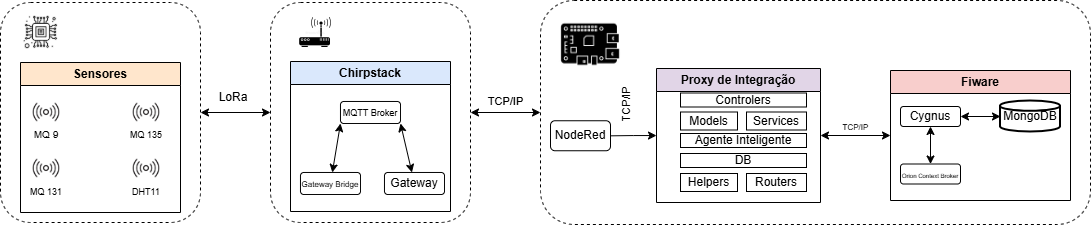
\includegraphics[width=0.9\textwidth]{Projeto-Mestre-Tornei-diagrama.png}
\caption{Arquitetura do IQArMobi aprimorado -- Fluxo completo de dados
desde a captura pelos sensores até o processamento inteligente}
\label{fig:arquitetura}
\end{figure}

O projeto baseia-se nos seguintes conceitos fundamentais:

\textbf{IoT e RTOS:} Utilização de sensores conectados (MQ-9, MQ-131,
MQ-138, DHT11) via LoRaWAN com sistemas de tempo real para garantir
respostas determinísticas \cite{reddy2023}.

\textbf{Aprendizado de Máquina:} Algoritmos para predição temporal e
detecção de anomalias em dados ambientais, implementados no Agente
Inteligente que processa dados via Node-RED e FIWARE.

\textbf{Arquitetura Distribuída:} Integração desde sensores (borda) até
nuvem (FIWARE, MongoDB), com middleware ChirpStack/Node-RED para
orquestração de dados.

\textbf{Agente Inteligente:} Sistema autônomo com capacidades preditivas
e resposta automatizada, diferencial da proposta para o IQArMobi.

\section*{4. TRABALHOS RELACIONADOS}

Trabalhos relevantes incluem: \cite{mokrani2019} apresenta panorama de
IoT para monitoramento; \cite{kumar2023} propõe solução urbana
inteligente; \cite{cunha2024} demonstra arquitetura LoRaWAN/FIWARE;
\cite{benammar2018} desenvolve plataforma modular; \cite{septian2022}
implementa sistema FreeRTOS.

\textbf{Lacuna identificada:} Poucos trabalhos integram capacidades
preditivas de IA com resposta automatizada em tempo real, especialmente
adaptados para a região amazônica.

\section*{5. METODOLOGIA}

A pesquisa adotará uma abordagem \textbf{Design Science Research (DSR)}, 
focada no desenvolvimento e avaliação de um artefato tecnológico - o agente inteligente IQArMobi aprimorado. 
A metodologia será estruturada em ciclos iterativos de construção e avaliação, conforme ilustrado na Figura 2.


\begin{figure}[h]
\centering
\begin{tikzpicture}[
    node distance=1cm and 2cm,
    etapa/.style={rectangle, draw, fill=blue!20, text width=2.8cm, 
                  align=center, minimum height=1.3cm, font=\footnotesize},
    seta/.style={->, thick, blue!70},
    tempo/.style={rectangle, draw=none, fill=none, text width=1.8cm, 
                  align=center, font=\tiny}
]

% Etapas
\node[etapa] (etapa1) {Etapa 1\\Análise de\\Requisitos};
\node[etapa, right=of etapa1] (etapa2) {Etapa 2\\Sistema\\Embarcado};
\node[etapa, right=of etapa2] (etapa3) {Etapa 3\\Agente\\Inteligente};
\node[etapa, below=of etapa2] (etapa4) {Etapa 4\\Integração\\e Testes};
\node[etapa, right=of etapa4] (etapa5) {Etapa 5\\Validação\\em Campo};

% Tempos
\node[tempo, below=0.2cm of etapa1] {Meses\\1--4};
\node[tempo, below=0.2cm of etapa2] {Meses\\5--9};
\node[tempo, below=0.2cm of etapa3] {Meses\\10--14};
\node[tempo, below=0.2cm of etapa4] {Meses\\15--20};
\node[tempo, below=0.2cm of etapa5] {Meses\\21--24};

% Setas principais
\draw[seta] (etapa1) -- (etapa2);
\draw[seta] (etapa2) -- (etapa3);
\draw[seta] (etapa3) -- (etapa4);
\draw[seta] (etapa4) -- (etapa5);

% Seta de feedback
\draw[seta, dashed, red!70] (etapa5) to[bend right=35] 
     node[above, midway, font=\tiny, text=red] {Feedback} (etapa1);

\end{tikzpicture}
\caption{Fluxograma da Metodologia -- Etapas sequenciais com 
         feedback para refinamentos contínuos}
\label{fig:metodologia}
\end{figure}

\subsection*{5.1 Abordagem Geral}

A metodologia seguirá o paradigma \textbf{pesquisa-desenvolvimento}, 
combinando métodos quantitativos para avaliação de desempenho e métodos qualitativos para validação em contexto real.
 O processo será dividido em três macroetapas interligadas:

\subsection*{5.2 Ciclo de Desenvolvimento do Artefato}

\textbf{Etapa 1: Problematização e Especificação de Requisitos}
\begin{itemize}
    \item \textbf{Revisão bibliográficas}: Revisão sistemática das soluções existentes de monitoramento 
    de qualidade do ar em smart campus, identificando lacunas e oportunidades de aprimoramento.
    \item \textbf{Especificação de Requisitos}: Definição dos requisitos funcionais e não-funcionais baseada em estudos 
    de caso de campi universitários da região amazônica, considerando particularidades climáticas e operacionais.
    \item \textbf{Projeto da Arquitetura}: Elaboração da arquitetura distribuída integrando IoT, edge computing e cloud 
    computing, com definição dos protocolos de comunicação (LoRaWAN, MQTT) e interfaces.
\end{itemize}

\textbf{Etapa 2: Projeto e Implementação}
\begin{itemize}
    \item \textbf{Desenvolvimento da Camada Física}: Implementação dos nós sensores com microcontroladores ESP32 e
     sensores especializados (MQ-9, MQ-131, MQ-135, DHT11), incorporando RTOS para garantia de tempo real.
    \item \textbf{Implementação do Middleware}: Configuração da infraestrutura LoRaWAN com ChirpStack, integração com 
    FIWARE para orquestração de dados, e desenvolvimento de serviços em Node-RED para pré-processamento.
    \item \textbf{Desenvolvimento do Agente Inteligente}: Implementação dos algoritmos de aprendizado de máquina para 
    predição temporal, detecção de anomalias e mecanismos de decisão 
    para resposta automatizada.
\end{itemize}

\textbf{Etapa 3: Integração e Validação}
\begin{itemize}
    \item \textbf{Integração Sistêmica}: Unificação dos componentes desenvolvidos, garantindo interoperabilidade entre 
    hardware, middleware e software inteligente.
    \item \textbf{Testes de Laboratório}: Avaliação controlada do sistema integrado, verificando 
    desempenho, confiabilidade e atendimento aos requisitos de tempo real.
    \item \textbf{Validação em Ambiente Real}: Implantação piloto em campus universitário, 
    com coleta contínua de dados e monitoramento do comportamento do sistema em condições operacionais.
\end{itemize}

\subsection*{5.3 Métodos de Avaliação}

\textbf{Avaliação Técnica}
\begin{itemize}
    \item \textbf{Métricas de Desempenho}: Acurácia preditiva, recall na detecção de anomalias, tempo de resposta, 
    consumo energético e confiabilidade da comunicação.
    \item \textbf{Testes de Estresse}: Submissão do sistema a condições extremas de operação para 
    verificação de robustez e tolerância a falhas.
    \item \textbf{Benchmarking Comparativo}: Análise comparativa do desempenho do IQArMobi aprimorado frente 
    à versão original e outras soluções do estado da arte.
\end{itemize}

\textbf{Avaliação em Contexto}
\begin{itemize}
    \item \textbf{Estudos de Caso}: Implementação em diferentes cenários do campus 
    (laboratórios, salas de aula, áreas externas) para avaliação contextualizada.
    \item \textbf{Análise de Usabilidade}: Avaliação da interface e mecanismos de alerta junto 
    à comunidade acadêmica, considerando clareza e utilidade das informações.
    \item \textbf{Avaliação de Impacto}: Análise do contributo do sistema para 
    a gestão ambiental do campus e para a conscientização da comunidade sobre qualidade do ar.
\end{itemize}

\subsection*{5.4 Coleta e Análise de Dados}

Os dados serão coletados através de:
\begin{itemize}
    \item \textbf{Sensores IoT}: Leitura contínua de parâmetros de qualidade do ar (CO, O3, NO2, temperatura, umidade)
    \item \textbf{Logs do Agente Inteligente}: Registros de predições, detecções de anomalias e ações automatizadas
    \item \textbf{Logs do Sistema}: Registro de desempenho, eventos e respostas automatizadas
    \item \textbf{Questionários e Entrevistas}: Feedback da comunidade acadêmica sobre utilidade e usabilidade
\end{itemize}

A análise utilizará métodos estatísticos para validação de hipóteses técnicas e 
métodos qualitativos para interpretação dos resultados contextuais.

\section*{6. RESULTADOS ESPERADOS E CONTRIBUIÇÕES}

Espera-se, como resultado central, a disponibilização de uma versão
aprimorada do IQArMobi, capaz de realizar monitoramento contínuo da
qualidade do ar com capacidades de predição temporal e resposta
automatizada em tempo real, integrada a uma arquitetura IoT escalável e
adaptada ao contexto da região amazônica. A solução deverá apresentar
ganhos mensuráveis em termos de acurácia preditiva, redução do tempo
de resposta a eventos críticos e eficácia dos mecanismos de
notificação e mitigação, quando comparada à versão original do sistema.

\textbf{Do ponto de vista científico, são esperadas contribuições na forma de:}
\begin{itemize}
    \item Modelos e estratégias de aprendizado de máquina para previsão
    de qualidade do ar em contexto amazônico, considerando
    características sazonais e padrões locais de poluição.
    \item Avaliação experimental da integração entre sistemas
    operacionais de tempo real, middleware IoT (LoRaWAN, FIWARE) e
    algoritmos de IA em um cenário de missão crítica de monitoramento
    ambiental
    \item Publicações em periódicos e eventos da área de Computação
    Aplicada, Inteligência Artificial e Internet das Coisas, destacando
    os resultados de predição, detecção de anomalias e resposta
    automática.
\end{itemize}

\textbf{Do ponto de vista tecnológico e social, são esperadas contribuições como:}
\begin{itemize}
    \item Um protótipo funcional de agente inteligente para monitoramento
    e gestão da qualidade do ar em campus universitário, potencialmente
    replicável para outros ambientes urbanos e institucionais.
    \item Uma arquitetura de referência, documentada, para integração de
    sensores, comunicação LoRaWAN, processamento em borda e nuvem, e
    tomada de decisão automatizada em tempo real.
    \item Subsídios para a gestão institucional e para ações de saúde e
    meio ambiente, por meio de dados e alertas que apoiem decisões
    relacionadas à exposição da comunidade acadêmica a poluentes
    atmosféricos.
\end{itemize}

\section*{7. REFERÊNCIAS BIBLIOGRÁFICAS}

\bibliography{./referencias}
\bibliographystyle{abntex2-alf} % Define o estilo ABNT para
                              % formatar a lista

\section*{8. POSSÍVEIS ORIENTADORES}

\begin{enumerate}
    \item \textbf{Prof. Dr. Elton Rafael Alves} -- Inteligência
    Computacional, Mineração de Dados, Inteligência Artificial,
    Sistemas Embarcados e Descargas Atmósfericas.
    
   % \item \textbf{Prof. Dr. Adam Dreyton Ferreira dos Santos} - Inteligência Artificial, 
   % Aprendizado de máquina, Visão computacional e Computação Aplicada à Engenharia.
\end{enumerate}

\vspace{1cm}

\end{document}